\documentclass[t]{beamer}

% Load general definitions
% Preamble file - general definitions, package loading, etc.

%=================================
% Load packages
\usepackage{amssymb,amsmath}
\usepackage{graphicx}
\usepackage{url}
\usepackage{tikz}
\usetikzlibrary{mindmap,trees,arrows}
\usepackage{fancyvrb}
\usepackage[english]{babel}
\usepackage[latin1]{inputenc}
\usepackage{subfigure}
\usepackage{times}
\usepackage[T1]{fontenc}
\usepackage{cancel}
\usepackage{color}
\usepackage{listings}

%=================================
% Set mode
\mode<presentation>
{
	\usetheme{Madrid}
	\usecolortheme{whale}
	\useoutertheme{infolines}
	\setbeamercovered{invisible}
}

% Get rid of nav bar
\beamertemplatenavigationsymbolsempty

% Insert frame number at bottom of the page.
\usefoottemplate{\hfil\tiny{\color{black!90}\insertframenumber}} 

%=================================
% Define new commands

\newcommand\Real{{\mathbb{R}}}
%\newcommand{\vi}{\vspace{0.6\baselineskip}}
%\newcommand{\goodgap}{\hspace{\subfigtopskip}\hspace{\subfigbottomskip}}


% Equation environments
\newcommand{\beq}{\begin{equation}}
\newcommand{\eq}{\end{equation}}
\newcommand{\beqs}{\begin{equation*}}
\newcommand{\eqs}{\end{equation*}}
\newcommand{\beqn}{\begin{eqnarray}}
\newcommand{\eqn}{\end{eqnarray}}

% Bold variables
\newcommand{\mbf}[1]{\ensuremath{\mathbf{#1}}}

% Itemization
\newcommand{\bitem}{\begin{itemize}}
\newcommand{\eitem}{\end{itemize}}
\newcommand{\spitem}{\vskip 1em\item}
\newcommand{\bitems}{\begin{itemize}\item}
\newcommand{\benums}{\begin{enumerate}\item}
\newcommand{\eenum}{\end{enumerate}}

% color blocks
\newenvironment{colorblock}[2]{%
\setbeamercolor{block title}{#2}
\begin{block}{#1}}{\end{block}}

% Vertical spacing
\newcommand{\vone}{\vskip 1em}
\newcommand{\vhalf}{\vskip .5em}

% Frame environments
\newenvironment{ftst}[3][t]{%
\begin{frame}{environment=ftst,#1}
\frametitle{#2}
\framesubtitle{#3}}{\end{frame}}

\newenvironment{ftstf}[2]{
\begin{frame}[fragile,environment=ftstf]
\frametitle{#1}
\framesubtitle{#2}}{\end{frame}}

% colors
\definecolor{MyGray}{rgb}{0.5,0.5,0.5}
\definecolor{MyDBGray}{rgb}{0.1,0.1,0.4}
\definecolor{darkgreen}{rgb}{0,0.4,0}
\definecolor{black}{rgb}{0,0,0}
\def\defn#1{{\color{red} #1}}

% Footnote
\renewcommand{\thefootnote}{\alph{footnote}}

% Relaxed footnotes
\newcommand{\lfr}[1]{\let\thefootnote\relax\footnote{\tiny #1}}

% Verbatim environment - using FANCYVRB package
\DefineVerbatimEnvironment%
{rcode}{Verbatim}
{fontsize=\scriptsize}

% Verbatim environment - using LISTINGS package
%\lstnewenvironment{rcode} {\lstset{	language = R,
%									basicstyle = \scriptsize\ttfamily,
%									showspaces = false,
%									showstringspaces = false,
%									showtabs = false,
%									keywordstyle = \color{black}\bfseries,
%									commentstyle = \color{darkgreen},
%									numbers = none,
%									otherkeywords={	<-,
%													ggplot,
%													geom_boxplot,
%													facet_grid,
%													shapiro.test,
%													fligner.test,
%													glht,
%													with},
%									deletekeywords={data,
%													model,
%													residuals,
%													c,
%													axis,
%													default,
%													labels,
%													qq.text}}}%
%{}


% Specific definitions
\title[]{Design and Analysis of Experiments}
\subtitle[]{00 - Course Intro}
\author[]{Felipe Campelo\\{\footnotesize http://orcslab.cpdee.ufmg.br/}}
\institute{Graduate Program in Electrical Engineering}
\date{\scriptsize Belo Horizonte\\August 2018}

\begin{document}

% cover page
\setbeamertemplate{footline}{}
\begin{frame}
\begin{flushright}

\includegraphics[width=.25\textwidth]{../figs/principal_completa3_ufmg}
\end{flushright}
  \titlepage
  \begin{tikzpicture}[remember picture,overlay]
  \node[anchor=south east,xshift=-5pt,yshift=122pt] at (current page.south east) {\tiny Version 2.12.2018b};
  \node[anchor=south west,yshift=0pt] at (current page.south west) {
\includegraphics[width=.15\textwidth]{../figs/by-nc-sa.png}};
  \end{tikzpicture}  
\end{frame}

% quotation page
  \begin{frame}[b]
		\frametitle{}
\begin{columns}[T]
\column{0.8\textwidth}
\flushright{\small ``\textit{I didn't want to just know names of things.\\I remember really wanting to know how it all worked.}''\\ \vspace{3em} Elizabeth Blackburn (1948 -- )\\Australian-American Molecular Biologist\\\ \\}
\column{0.2\textwidth}
\begin{tikzpicture}[remember picture,overlay]
\node[anchor=south east,yshift=15pt,xshift=0pt] at (current page.south east) {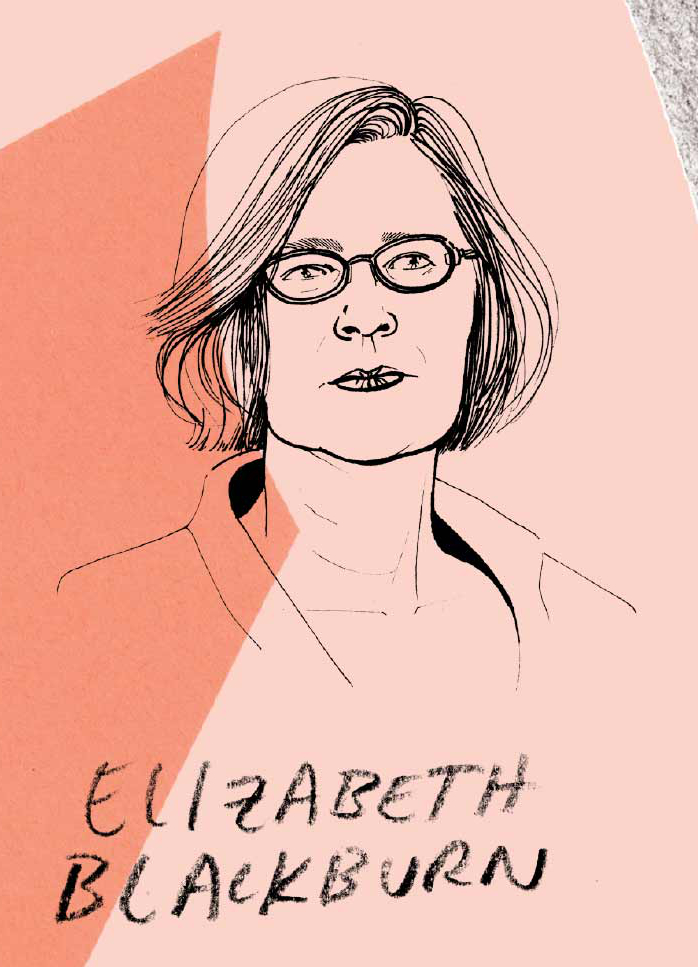
\includegraphics[width=\textwidth]{../figs/ElizabethBlackburn-bySamanthaHahn.jpg}};
\end{tikzpicture}
\end{columns}
\vskip .5em
\lfr{Image by Samantha Hahn: \url{https://awomensthing.org/blog/tag/science/}}
\end{frame}

% Main slides
\begin{ftst}
{Course Overview}
{Objectives}
\bitems To develop basic skills in designing experiments, defining and testing hypotheses, and performing statistical data analyses within one's field of interest;
\spitem By the end of this course, the student should be able to:
\bitems Plan experiments related to his/her work;
\item Perform appropriate statistical analyses of the data obtained from the experiment;
\item Develop sound conclusions based on the available data;
\item Identify the problems and limitations of his/her own experiments, and suggest improvements;
\item Perform critical interpretations of other experimental methodologies and results reported in the literature.
\eitem\eitem
\end{ftst}

%=====

\begin{ftst}
{Course Overview}
{Course Structure}
\bitems Lectures: discussions about several aspects and techniques for design and analyses of experiments. Theory and application examples;
\spitem Computational case studies; 
\spitem Final project presentations;
\spitem Written exam;
\spitem Tutoring;
\eitem
\end{ftst}

%=====

\begin{ftst}
{Course Overview}
{Course Structure}
\begin{block}{Evaluation criteria}
	\begin{center}
		\small
		\begin{tabular}{cccc} \hline
			\textbf{Item}	& \textbf{Type}	&\textbf{Grades}\\
			\hline
			Case studies		& Short group projects		&35\\
			Written exam		& Written exam	&40\\
			Final Project		& Report and presentation		&25\\
			\hline
		\end{tabular}
	\end{center}
\end{block}

\begin{block}{Other relevant Information}
	\bitems Lectures slides, example R files, data, etc. available at \\
	{\small \url{http://git.io/v3Kh8}}
	\spitem Office hours: depends on the week. Please drop me a message to check availability.
	\spitem Software/services used: R ({\scriptsize\url{http://cran.r-project.org/}}),\\Github ({\scriptsize\url{http://github.com/}}).
	\eitem
\end{block}
\end{ftst}

%=====

\begin{ftst}
{Course Overview}
{Course Bibliography}
\textbf{Main}:\\
{\footnotesize
\bitems Felipe Campelo (2018), \textit{Lecture Notes on Design and Analysis of Experiments}. Online: \url{http://git.io/v3Kh8} Version 2.12; Creative Commons BY-NC-SA 4.0.
\item D.C. Montgomery, G.C. Runger (2010), \textit{Applied Statistics and Probability for Engineers}, John Wiley \& Sons.
\eitem}
\vhalf
\textbf{Additional}:
{\footnotesize
\bitems D.C. Montgomery (2012), \textit{Design and Analysis of Experiments}, Wiley.
\item Michael J. Crawley (2007), \textit{The R Book}, Wiley.
\item B. Caffo (2015), \textit{Statistical inference for data science}, LeanPub - {\small\url{https://leanpub.com/LittleInferenceBook/}}
\item J.J. Faraway (2002), \textit{Practical Regression and Anova using R} - {\small\url{http://goo.gl/ewMWL}}
\item D. Wiens (2005), \textit{Introduction to Design and Analysis of Experiments} - {\small\url{http://goo.gl/hZXg1}}
\eitem}
\end{ftst}

%=====

\begin{ftst}
{Course Overview}
{Required / Desired background}
This is a course on \textit{applied} experimental design and analysis. As such, a large portion of the course is dedicated to case studies in which the student will design experiments, collect (simulated) data, perform inference and report his or her analysis.
\vone
It is \textbf{strongly reccomended} that the student should complete the free online course  \textit{R Programming}\footnote{{\scriptsize\url{https://www.coursera.org/course/rprog}}} \textbf{before the end of the second week} of the semester (except if the student is already fluent in R).
\vone
It is also \textbf{strongly reccomended} that the student should complete the free online course  \textit{Reproducible Research}\footnote{{\scriptsize\url{https://www.coursera.org/course/repdata}}} \textbf{before the end of the first month} of the semester (except if the student is already capable of writing reports using R Markdown).
\end{ftst}

%=====

\begin{ftstf}{About this material}{Conditions of use and referencing}
\centering\footnotesize This work is licensed under the Creative Commons CC BY-NC-SA 4.0 license\\(Attribution Non-Commercial Share Alike International License version 4.0).\\
\vhalf
\url{http://creativecommons.org/licenses/by-nc-sa/4.0/}\\
\vone
\footnotesize Please reference this work as:\\
\footnotesize \flushleft Felipe Campelo (2018), \textit{Lecture Notes on Design and Analysis of Experiments}.\\Online: {\scriptsize\url{https://github.com/fcampelo/Design-and-Analysis-of-Experiments}}\\
Version 2.12. Creative Commons BY-NC-SA 4.0.\\

\begin{Verbatim}[fontsize=\tiny]
    @Misc{Campelo2018,
      title={Lecture Notes on Design and Analysis of Experiments},
      author={Felipe Campelo},
      howPublished={\url{https://github.com/fcampelo/Design-and-Analysis-of-Experiments}},
      year={2018},
      note={Version 2.12. Creative Commons BY-NC-SA 4.0.},
    }
\end{Verbatim}

\begin{tikzpicture} [remember picture,overlay]
\node[anchor=south,yshift=0pt] at (current page.south){ \includegraphics[width=.2\textwidth]{../figs/CCSomerights.png}};
\end{tikzpicture}
\end{ftstf}


%=====

\end{document}